\chapter{Thực nghiệm, kết quả và thảo luận}
\label{ch:thuc-nghiem}
% Đề mục 4: Môi trường chạy; ma trận đối đầu; win/draw/loss; độ trễ/chi phí; learning curves;
% ablations; minh họa ván cờ, phân tích thất bại. Chỉ ghi số liệu đã chạy thật (đề mục 5).

\section{Môi trường thực nghiệm}
Báo cáo tách ba loại bằng chứng. Thứ nhất là benchmark trên thế cờ, trong đó mỗi quan sát là một thế và mục tiêu là đo chi phí hoặc tính nhất quán. Thứ hai là đối đầu, trong đó mỗi quan sát là một ván và đơn vị ghép cặp là khai cuộc. Thứ ba là log huấn luyện: mỗi vòng có thể thay trọng số và đối thủ dùng để kiểm tra, nên điểm qua các vòng không tạo thành đường so sánh trước một đối thủ cố định. Mã trong nhánh đang làm việc có thể mới hơn phiên bản từng ghi log.

\begin{table}[H]
\centering\small
\begin{tabularx}{\textwidth}{@{}lXl@{}}
\toprule
Nguồn & Đơn vị so sánh & Quy mô \\
\midrule
A1/A2/A7 & So sánh thao tác AlphaBeta trên tập thế cờ & 50 / 10 / 10 thế \\
A3/A4 & UCT gặp L2 và L3, ghép theo khai cuộc & 1.600 / 800 ván \\
Arena cũ & Sáu cấu hình từ L1 đến hai phiên bản L5 & 1.500 ván \\
A5 & L5, L6 và các cấu hình L7, 200 ván/cặp & 2.200 ván \\
Huấn luyện L6 & Episode tự đấu và đánh giá định kỳ & 49.920 episode \\
Huấn luyện L8 & Tự đấu và đấu kiểm tra ứng viên & 50 vòng \\
L8 gặp L7 & Cùng 200 mô phỏng, 10 khai cuộc đổi màu & 20 ván \\
L8 gặp L3 & L8 200 mô phỏng, L3 độ sâu 6 & 40 ván \\
\bottomrule
\end{tabularx}
\caption{Các nguồn đã có số liệu. Một số nguồn có thể dùng chung khai cuộc; không cộng chúng để suy ra cỡ mẫu độc lập.}
\end{table}

\section{Giải đấu chính}
\subsection{Ma trận đối đầu --- chế độ A (thời gian/nước)}
\subsection{Ma trận đối đầu --- chế độ B (ngân sách cố định)}
\subsection{Thắng / hoà / thua và xếp hạng Elo}
Arena cũ chạy sáu cấu hình, mỗi tác tử có 500 ván. Hai cấu hình L5 là hai phiên bản lịch sử. L3 của lượt này ghi độ sâu 3 trong nhãn, nên kết quả không dùng làm mốc trực tiếp cho L3 độ sâu 6 trong A5. Toàn bộ trận lịch sử chỉ có tổng kết và số nước; dữ liệu này hỗ trợ bảng xếp hạng và phân tích theo màu nhưng không hỗ trợ gán lỗi chiến thuật cho từng nước.
\begin{center}\small
\begin{tabular}{@{}lrrrrr@{}}
\toprule
Tác tử & Ván & Thắng & Hòa & Thua & Điểm \\
\midrule
L3 AB d3 & 500 & 404 & 1 & 95 & 80,9\% \\
L5 v2 & 500 & 369 & 4 & 127 & 74,2\% \\
L2 rule & 500 & 327 & 2 & 171 & 65,6\% \\
L5 v1 & 500 & 296 & 1 & 203 & 59,3\% \\
L4 MCTS200 & 500 & 96 & 0 & 404 & 19,2\% \\
L1 random & 500 & 4 & 0 & 496 & 0,8\% \\
\bottomrule
\end{tabular}
\end{center}

\begin{table}[H]
\centering\small
\begin{tabular}{@{}lrrrrrr@{}}
\toprule
Tác tử & L1 & L2 & L3 d3 & L4 & L5 v1 & L5 v2 \\
\midrule
L1 random  & --- & 0 & 0 & 4 & 0 & 0 \\
L2 rule    & 100 & --- & 39 & 100 & 55 & 34 \\
L3 AB d3   & 100 & 61 & --- & 100 & 86 & 57,5 \\
L4 MCTS200 & 96 & 0 & 0 & --- & 0 & 0 \\
L5 v1      & 100 & 45 & 14 & 100 & --- & 37,5 \\
L5 v2      & 100 & 66 & 42,5 & 100 & 62,5 & --- \\
\bottomrule
\end{tabular}
\caption{Ma trận điểm phần trăm của tác tử ở hàng trước tác tử ở cột, tái tính từ arena cũ. Mỗi ô có 100 ván.}
\label{tab:arena-lich-su}
\end{table}

Bảng~\ref{tab:arena-lich-su} cho thấy vì sao cần xem cặp đấu bên cạnh điểm tổng.
L4 thắng 96/100 trước L1, nhưng không ghi điểm trước bốn cấu hình còn lại. Điểm tổng
19,2\% của L4 vì thế chủ yếu phản ánh trận đấu với L1. Với L5, thay phiên bản cải thiện
điểm trước L3 từ 14,0\% lên 42,5\% và trước L2 từ 45,0\% lên 66,0\% trong cùng giải.
Điều quan sát được là tác động của việc thay checkpoint. Ma trận không tự tách được
ảnh hưởng của dữ liệu, thời lượng huấn luyện hay siêu tham số giữa hai phiên bản.
Trong 1.500 ván lịch sử, X thắng 828, O thắng 668 và hòa 4; chênh lệch
tỷ lệ thắng thuần là 10,67 điểm phần trăm. Đây là hiệu ứng gộp theo cơ cấu cặp đấu cũ.
\subsubsection{Elo và khoảng tin cậy của thứ hạng}

\section{Chi phí tính toán}
Cộng đồng hồ của nước tự đấu trong log L8 cho khoảng 8 giờ 16 phút; cộng đồng hồ nước đấu kiểm tra cho khoảng 2 giờ 23 phút. So với 44.327,952 giây của lượt chạy, hai tổng lần lượt chiếm khoảng 67\% và 19\%.
Phần thời gian còn lại gồm cập nhật trọng số, chuẩn bị mẫu, lưu checkpoint và các chi phí
điều phối ngoài phép đo từng nước. Log chưa tách được chi phí của từng thành phần trong phần còn lại. Chúng phản ánh nơi chi phí tập trung trong lượt đã chạy. Không dùng chênh lệch giữa hai lượt huấn luyện có trạng thái hệ thống khác nhau để kết luận Cython nhanh hay chậm hơn. Bản mới có gom suy luận giữa ván và ghi thời gian từng pha. Đây là thay đổi của mã; chưa có phép đo đối chứng GPU đủ để báo tỷ lệ tăng tốc toàn vòng.

\section{Huấn luyện}
\subsection{Cấp 5 --- học có giám sát}
Các log SL v1, v2 và v3 lần lượt ghi 30, 30 và 60 epoch. Ở từng lượt, phép tra cứu tối thiểu
dựa trên validation loss ghi nhận epoch 30, 28 và 55. Với SL v3, validation loss thấp nhất
là 1,4723 và giá trị ở epoch cuối là 1,4758. Đó là độ đo huấn luyện, còn sức chơi phải
đối chiếu riêng theo checkpoint và đối thủ.
\begin{center}\small
\begin{tabular}{@{}lrrrr@{}}
\toprule
Mạng & Số epoch & Epoch tốt nhất & Val loss tốt nhất & Val loss cuối \\
\midrule
SL v1 & 30 & 30 & 2,1566 & 2,1566 \\
SL v2 & 30 & 28 & 1,6020 & 1,7095 \\
SL v3 & 60 & 55 & 1,4723 & 1,4758 \\
\bottomrule
\end{tabular}
\end{center}
\begin{center}\small
\begin{tabular}{@{}llrrr@{}}
\toprule
Checkpoint & Đối thủ & Ván & W/D/L & Điểm \\
\midrule
SL v1 & L2 & 100 & 40/0/60 & 40,0\% \\
SL v1 & L3 & 100 & 5/0/95 & 5,0\% \\
SL v2 & L2 & 100 & 66/0/34 & 66,0\% \\
SL v2 & L3 & 100 & 19/3/78 & 20,5\% \\
SL v3 & L2 & 100 & 63/6/31 & 66,0\% \\
SL v3 & L3 & 100 & 19/4/77 & 21,0\% \\
RL v2 best & L2 & 100 & 72/1/27 & 72,5\% \\
RL v2 best & L3 & 100 & 25/5/70 & 27,5\% \\
RL v3 best & L2 & 100 & 79/4/17 & 81,0\% \\
RL v3 best & L3 & 100 & 33/8/59 & 37,0\% \\
RL v3 last & L2 & 100 & 81/1/18 & 81,5\% \\
RL v3 last & L3 & 100 & 33/7/60 & 36,5\% \\
\bottomrule
\end{tabular}
\end{center}
\subsubsection{Top-1 và top-3 trên tập giữ riêng}
\subsection{Cấp 6 và cấp 8 --- learning curve}
L6 dùng REINFORCE từ checkpoint SL. Lượt v3 ghi 49.920 episode và hơn 1,5 triệu nước.
Điểm cuối trong log huấn luyện là 78,5\% trước L2 và 26,0\% trước AlphaBeta.
Kết quả trước L2 và L3 phản ánh sức chơi của một checkpoint với đối thủ cụ thể. Trong phép đánh giá riêng, RL v3 best đạt 81,0\% trước L2 và 37,0\% trước L3, trong khi SL v3 đạt 66,0\% và 21,0\%. Trong lượt huấn luyện RL v3, đánh giá vòng cuối ghi 78,5\% trước L2 và 26,0\% trước L3. Các cặp số này đến từ checkpoint và phép đánh giá khác nhau, nên không gộp thành một đường tăng đơn điệu. Chưa có đối chứng nhiều seed giữ nguyên ngân sách để tách riêng tác động của điều kiện khởi tạo.

\begin{table}[H]
\centering\small
\begin{tabular}{@{}rrr@{}}
\toprule
Episode & Điểm trước L2 & Điểm trước L3 \\
\midrule
5.120  & 53,5\% & 19,0\% \\
10.112 & 74,0\% & 17,5\% \\
15.104 & 69,5\% & 18,0\% \\
20.096 & 76,5\% & 31,0\% \\
25.088 & 78,0\% & 30,0\% \\
30.080 & 70,5\% & 31,0\% \\
35.072 & 80,0\% & 35,5\% \\
40.064 & 74,5\% & 30,5\% \\
45.056 & 78,0\% & 33,0\% \\
49.920 & 78,5\% & 26,0\% \\
\bottomrule
\end{tabular}
\caption{Các mốc đánh giá trong lượt REINFORCE v3. Mỗi điểm dùng 100 ván trước đối thủ tương ứng.}
\label{tab:rl-qua-moc}
\end{table}

Tại các mốc trong Bảng~\ref{tab:rl-qua-moc}, điểm cao nhất trước cả hai đối thủ rơi
vào episode 35.072; điểm trước L3 sau đó giảm 9,5 điểm phần trăm đến cuối lượt.
Vì các mốc đánh giá sử dụng các khai cuộc tạo từ seed theo mốc, sự dao động có thể do
cả thay đổi trọng số lẫn khác biệt của mẫu ván. Lấy checkpoint theo tiêu chí định trước
và đánh lại trên một tập giữ riêng sẽ giúp phân biệt hai khả năng.

Lượt \repoFile{20261124-160615_gpu-native} dùng CUDA và PUCT Cython, khởi tạo từ L5. Thiết lập gốc có 200 ván tự đấu mỗi vòng ở 400 mô phỏng/nước, 1.000 bước cập nhật và 100 ván kiểm tra ứng viên ở 200 mô phỏng/nước. Tổng thời gian là khoảng 12 giờ 19 phút. Máy ghi nhận Intel Core i7-11800H, NVIDIA RTX A2000 Laptop GPU, Python 3.13.16 và PyTorch 2.14.1 với CUDA 13.0. Seed là 2026. Lượt này chạy trước thay đổi gom suy luận giữa nhiều ván tự đấu.

\begin{center}\small
\begin{tabular}{@{}lrrr@{}}
\toprule
Vòng được duyệt & Ván kiểm tra & W/D/L & Điểm \\
\midrule
12 & 100 & 56/3/41 & 57,5\% \\
18 & 100 & 54/10/36 & 59,0\% \\
19 & 100 & 49/13/38 & 55,5\% \\
24 & 100 & 49/12/39 & 55,0\% \\
29 & 100 & 55/14/31 & 62,0\% \\
37 & 100 & 53/16/31 & 61,0\% \\
\bottomrule
\end{tabular}
\end{center}
Ứng viên được duyệt ở các vòng 12, 18, 19, 24, 29 và 37. Vòng 37 đạt 61,0\% trước bản đang giữ và là lần duyệt cuối; đây là checkpoint \repoFile{best.pt}. Ứng viên vòng 50 chỉ đạt 46,0\% trước bản đang giữ; file \repoFile{last.pt} vì vậy không phải checkpoint phục vụ kết quả cuối. Điểm gating của vòng 29 là 62,0\% trước bản đương nhiệm lúc đó. Không thể so trực tiếp 62,0\% với 61,0\% để xếp hai checkpoint, vì đối thủ đã đổi.
\begin{figure}[H]
\centering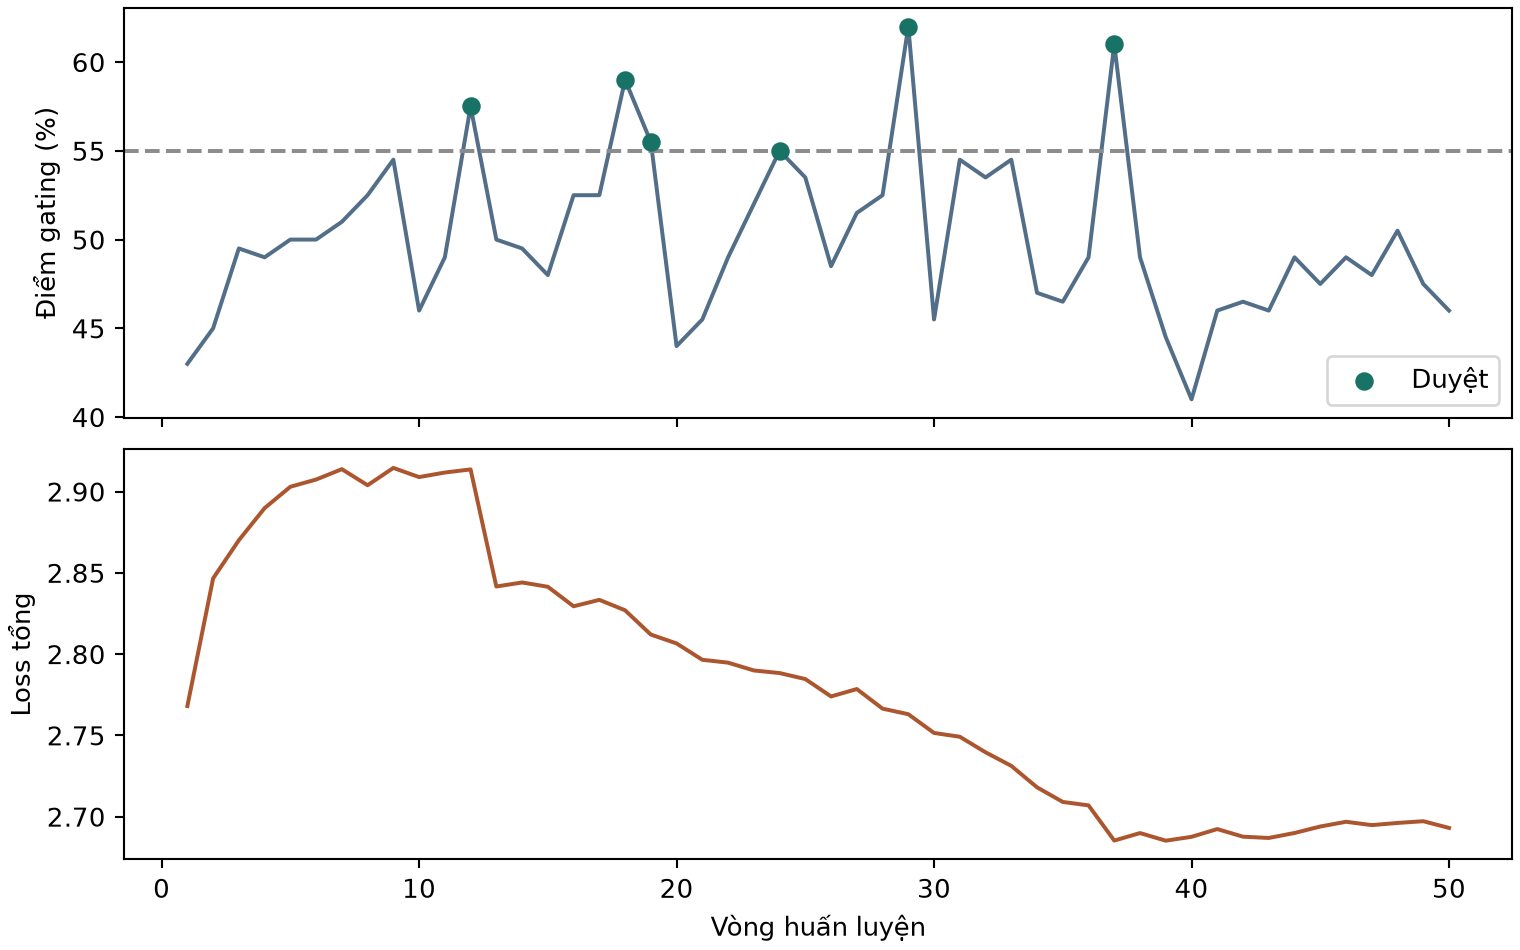
\includegraphics[width=.9\textwidth]{ban-mo-rong/hinh/l8.png}
\caption{Gating và loss trong 50 vòng. Điểm gating là điểm trước bản đương nhiệm ở từng thời điểm.}
\end{figure}

\section{Ablation và phân tích độ nhạy}
\subsection{A1, A2 --- cắt tỉa, sắp xếp nước, TT}
\begin{center}\small
\begin{tabular}{@{}llrrrr@{}}
\toprule
Nhóm & Cấu hình & Thế & Nút (P50) & ms (P50) & ms (P95) \\
\midrule
A1 & AB-prune & 50 & 39322 & 1273,1 & 5445,2 \\
A1 & AB-full & 50 & 802217 & 26576,0 & 42474,9 \\
A2 & AB-plain & 10 & 9106 & 990,0 & 993,1 \\
A2 & AB-order & 10 & 372 & 995,1 & 1049,0 \\
A2 & AB-order-tt & 10 & 486 & 994,9 & 1051,2 \\
A7 & AB-default & 10 & 366 & 578,2 & 2760,2 \\
A7 & AB-no-defense & 10 & 580 & 548,7 & 2358,0 \\
\bottomrule
\end{tabular}
\end{center}
A1 cho thấy số nút và thời gian trung vị cùng giảm khoảng 20 lần trong phép đo này. Giá trị ở gốc trùng trên cả 50 thế theo trường nhất quán của benchmark. Trường này đo giá trị gốc, không đếm số lần chọn cùng nước khi có nhiều nước đồng hạng. Với A2, số nút của hai cấu hình có sắp xếp thấp hơn rõ, trong khi thời gian trung vị xấp xỉ nhau. Vì các lượt chạy dùng ngân sách thời gian gần một giây, số nút ở đây phản ánh cả thứ tự, chi phí mỗi nút, và độ sâu có thể hoàn thành; không thể quy mức chênh lệch đó thành tăng tốc ở cùng độ sâu.
\subsection{A3, A4 --- số mô phỏng và kiểu rollout của MCTS}
\paragraph{Thiết lập.}
Cả hai thực nghiệm dùng cặp đấu \texttt{challengers\_vs\_baselines}: mỗi MCTS đấu với Cấp~2 (luật) và Cấp~3 (Alpha-Beta, độ sâu 4), seed gốc 2026, 100 khai cuộc, mỗi khai cuộc đấu hai ván đổi màu, nên mỗi cặp có 200 ván. A3 đổi số mô phỏng (100, 400, 1600, 6400; rollout \texttt{random}); A4 giữ 800 mô phỏng và đổi \texttt{rollout} giữa \texttt{random} và \texttt{light}. Thực nghiệm chạy bằng \texttt{notebooks/a3\_a4\_mcts.ipynb} với 4 worker; A3 gồm 1600 ván (22 phút), A4 gồm 800 ván (9 phút), không ván nào lỗi. Log nằm ở \texttt{runs/tournament/a3\_mcts\_sims/20261114-232353} và \texttt{runs/tournament/a4\_rollout/20261114-234556}. Cả hai run ghi \texttt{dirty: true} trong \texttt{meta.json} vì chạy khi working tree chưa commit (commit nền \texttt{27d6525}).

\paragraph{Kết quả A3.}
Điểm là $(\text{thắng}+0{,}5\times\text{hoà})/\text{tổng}$ của MCTS, kèm khoảng tin cậy Wilson 95\% (Bảng~\ref{tab:a3}, Hình~\ref{fig:a3}).
\begin{table}[H]
  \centering
  \footnotesize
  \setlength{\tabcolsep}{3pt}
  \begin{tabular}{rccrrr}
    \toprule
    \textbf{Mô phỏng} & \textbf{vs Cấp 2} & \textbf{vs Cấp 3} & \textbf{TB (ms)} & \textbf{p95 (ms)} & \textbf{mp/s} \\
    \midrule
    100  & 0{,}000 [0{,}000; 0{,}019] & 0{,}000 [0{,}000; 0{,}019] & 16{,}4   & 22{,}3   & \num{6112} \\
    400  & 0{,}000 [0{,}000; 0{,}019] & 0{,}000 [0{,}000; 0{,}019] & 68{,}9   & 85{,}3   & \num{5807} \\
    1600 & 0{,}000 [0{,}000; 0{,}019] & 0{,}000 [0{,}000; 0{,}019] & 298{,}5  & 359{,}6  & \num{5360} \\
    6400 & 0{,}075 [0{,}046; 0{,}120] & 0{,}020 [0{,}008; 0{,}050] & \num{1204.6} & \num{1467.2} & \num{5313} \\
    \bottomrule
  \end{tabular}
  \caption{A3: điểm của MCTS (rollout \texttt{random}) theo số mô phỏng, $n=200$ ván mỗi ô. Ở 6400 mô phỏng: 15 thắng/185 thua trước Cấp~2 và 4 thắng/196 thua trước Cấp~3; các mức còn lại thua toàn bộ 200 ván.}
  \label{tab:a3}
\end{table}
\begin{figure}[H]
  \centering
  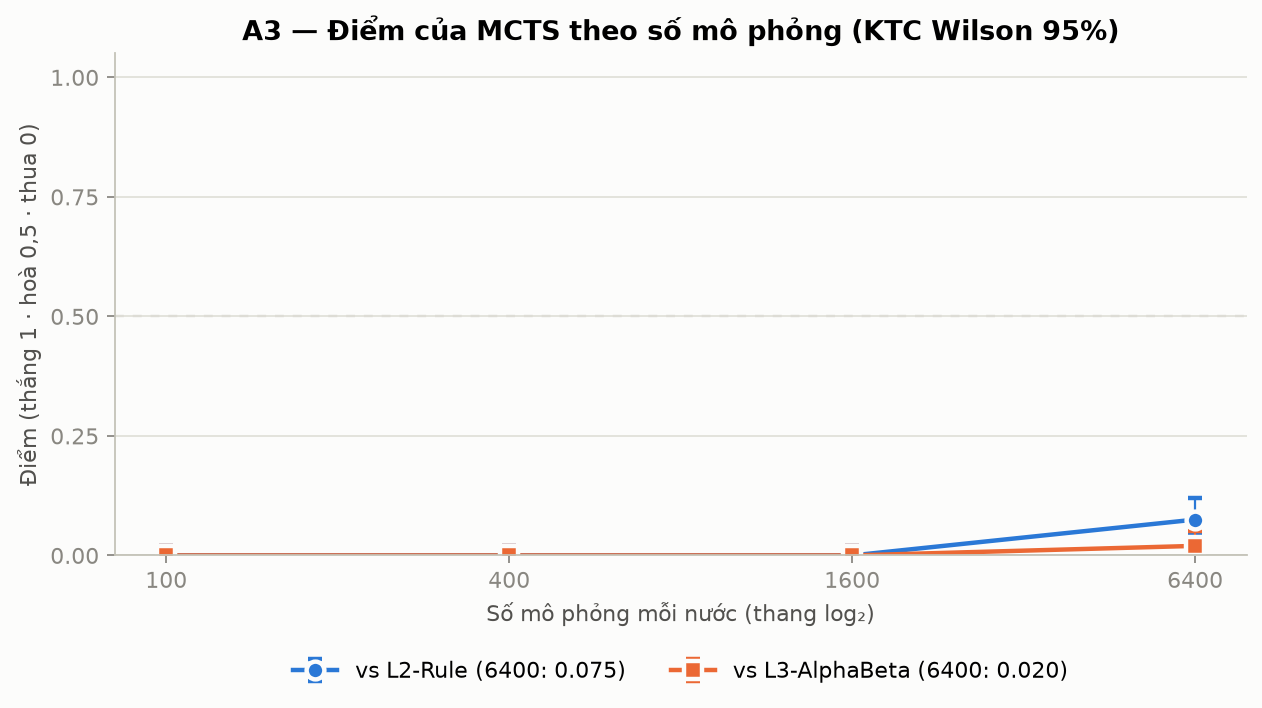
\includegraphics[width=.8\textwidth]{thuc-nghiem/a3_diem_theo_sims.png}
  \caption{A3: điểm của MCTS theo $\log_2$ số mô phỏng, có khoảng tin cậy Wilson 95\%.}
  \label{fig:a3}
\end{figure}
Ở từng mức 100, 400 và 1600 mô phỏng, MCTS thua toàn bộ 400 ván. Chỉ ở 6400 mô phỏng mới có ván thắng: bước tăng cuối 1600$\rightarrow$6400 đạt $+0{,}075$ trước Cấp~2 với hai khoảng tin cậy tách rời, còn trước Cấp~3 là $+0{,}020$ và hai khoảng chồng lấn. Số mô phỏng/giây giảm nhẹ từ khoảng 6100 xuống 5300 khi cây lớn hơn. Thời gian mỗi nước tăng gần tuyến tính theo số mô phỏng, tới trung bình 1,2 giây ở 6400.

\paragraph{Kết quả A4.}
Ở 800 mô phỏng, cả \texttt{random} lẫn \texttt{light} đều thua toàn bộ 400 ván (điểm $0{,}000$, Wilson [0,000; 0,019], trước cả hai đối thủ), nên \emph{không phân biệt được hai kiểu rollout} qua điểm số. Hai kiểu khác nhau rõ về chi phí: \texttt{random} mất 147,2 ms/nước (p95 177,8 ms; 5435 mô phỏng/s), \texttt{light} mất 551,7 ms/nước (p95 745,8 ms; 1450 mô phỏng/s), tức chậm khoảng 3,7 lần. (Dòng ``tốt hơn: MCTS-random'' trong notebook chỉ là so sánh hai số bằng nhau, không nên dùng làm kết luận.)

\paragraph{Thảo luận và kiểm tra.}
Phân tích ván gợi ý rằng một nguyên nhân là thiếu nhìn xa về chiến thuật: MCTS không chặn một ba hở trên đường chéo, đối thủ đi tiếp thành tứ hở và thắng; để thấy sự cố này cần cây sâu khoảng 4 ply (đi, đối thủ tạo tứ hở, đi, đối thủ thắng), trong khi 800 mô phỏng chia cho khoảng 40 nước gốc chỉ cho mỗi nước chừng 20 lượt thăm. Rollout \texttt{light} chỉ thắng/chặn \emph{ngay lập tức} nên không bù được chỗ này. Hai đối thủ lại có sẵn các luật chiến thuật (thắng ngay, chặn, đòn kép) nên khai thác điểm yếu đó. Các ván rất ngắn, trung bình khoảng 10--12 nước kể cả khai cuộc; toàn bộ
ván trong hai log đều kết thúc bằng năm quân liền. Vì thắng hoặc thua đến sớm,
tăng số mô phỏng có thể không có ích nếu cây chưa phân bổ đủ lượt thăm cho nhánh
phòng thủ hiếm. Đây là cơ chế phù hợp với phân tích nước đi, chưa phải một phép
đo riêng về độ sâu hữu hiệu của cây.

Điều này nghĩa là với ngân sách thực nghiệm, tăng số mô phỏng chỉ có tác dụng ở mức rất cao (6400), và A4 chưa đủ sức phân biệt. Để trả lời RQ1 đầy đủ, cần thêm đối thủ yếu hơn (ví dụ Random, hoặc Cấp~2 chỉ bật P1--P2) để điểm không dồn về 0, và đối chiếu với chế độ A (cùng thời gian mỗi nước). Đây là kết luận về mức độ thực nghiệm, chưa phải về MCTS nói chung.

\subsection{A5, A5b --- policy-only so với policy + MCTS; khởi tạo RL}
\subsubsection{A5: ảnh hưởng của PUCT khi giữ cùng mạng}
\begin{center}\small
\begin{tabular}{@{}llrrrr@{}}
\toprule
Tác tử & Đối thủ & Ván & W/D/L & Điểm & Wilson 95\% \\
\midrule
l5\_policy\_sl & l2\_rule & 200 & 130/2/68 & 65,50\% & [58,7\%; 71,7\%] \\
l5\_policy\_sl & l3\_alphabeta & 200 & 41/2/157 & 21,00\% & [15,9\%; 27,2\%] \\
l6\_policy\_rl & l2\_rule & 200 & 151/5/44 & 76,75\% & [70,4\%; 82,1\%] \\
l6\_policy\_rl & l3\_alphabeta & 200 & 54/19/127 & 31,75\% & [25,7\%; 38,5\%] \\
L7-PUCT[l5,100] & l3\_alphabeta & 200 & 88/9/103 & 46,25\% & [39,5\%; 53,2\%] \\
L7-PUCT[l5,200] & l3\_alphabeta & 200 & 104/26/70 & 58,50\% & [51,6\%; 65,1\%] \\
L7-PUCT[l5,400] & l3\_alphabeta & 200 & 105/34/61 & 61,00\% & [54,1\%; 67,5\%] \\
L7-PUCT[l5,800] & l3\_alphabeta & 200 & 118/32/50 & 67,00\% & [60,2\%; 73,1\%] \\
L7-PUCT[l5,200] & l2\_rule & 200 & 175/1/24 & 87,75\% & [82,5\%; 91,6\%] \\
L7-PUCT[l6,200] & l3\_alphabeta & 200 & 105/21/74 & 57,75\% & [50,8\%; 64,4\%] \\
L7-PUCT[l5,200] & l5\_policy\_sl & 200 & 191/0/9 & 95,50\% & [91,7\%; 97,6\%] \\
\bottomrule
\end{tabular}
\end{center}
Ở cùng đối thủ L3 và cùng mạng L5, policy trực tiếp đạt 21,0\%, còn L7 ở 200 mô phỏng đạt 58,5\%, chênh 37,5 điểm phần trăm. Ở trận trực tiếp, L7 tại ngân sách đó thắng L5 191/200 ván. So sánh cùng mạng làm rõ đóng góp của tìm kiếm trong cấu hình đã thử. Trong bốn mức mô phỏng, điểm trước L3 lên từ 46,25\% đến 67,0\%; log tổng hợp không có thời gian mỗi nước, do đó không xếp được các mức theo chi phí. Chênh giữa L7 dùng mạng L5 và mạng L6 ở 200 mô phỏng chỉ 0,75 điểm phần trăm; dữ liệu hiện có chưa đủ để xếp thứ tự hai mạng trong PUCT.
\begin{figure}[H]
\centering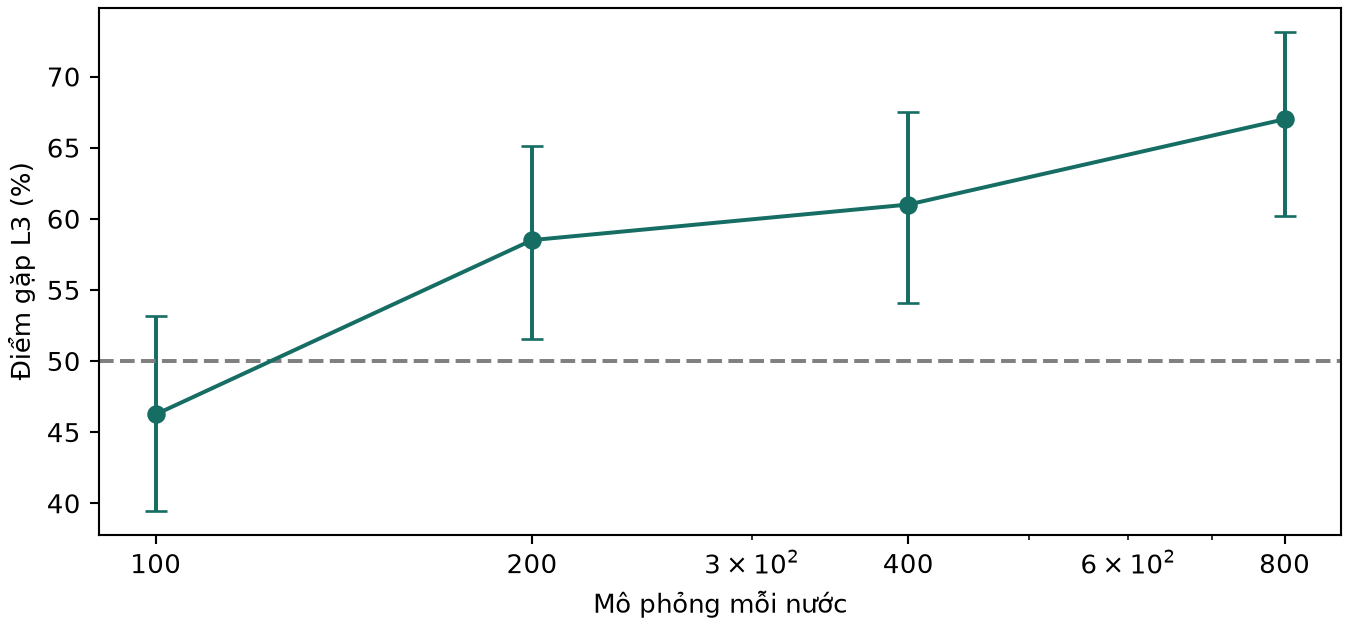
\includegraphics[width=.88\textwidth]{ban-mo-rong/hinh/a5.png}
\caption{Điểm L7 dùng mạng L5 trước L3 theo số mô phỏng. Đường ngang là mốc 50\%.}
\end{figure}
\subsubsection{A5b: đối chứng điều kiện khởi tạo qua nhiều seed}
\subsection{A6, A7 --- augmentation, trọng số hàm đánh giá}
\subsubsection{A6: so sánh tăng cường đối xứng}
\subsubsection{A7: đối chiếu giá trị ở gốc}
A7 cho thấy khi bỏ thành phần phòng thủ, giá trị gốc chỉ trùng trên 1/10 thế. Log tổng hợp này không cho biết có bao nhiêu nước được chọn thay đổi. Muốn suy ra mức tác động lên sức chơi cần kết quả đối đầu.
\subsection{E3 --- lợi thế đi trước}

\section{Trả lời câu hỏi nghiên cứu}
RQ1 có kết quả theo số mô phỏng, nhưng còn thiếu đối chứng cùng thời gian.
RQ2 có bằng chứng từ checkpoint SL/RL, A5 và đối đầu L8--L7. RQ3 được hỗ trợ bởi
benchmark A1; A2 cần đọc cùng ngân sách thời gian đã dùng. RQ4 có phân tích theo màu
trong hai đối sánh cụ thể, còn khảo sát tự đấu từng cấp chưa có số liệu chính thức.
Chương~\ref{ch:ket-luan} nêu mức độ trả lời của từng kết quả.

\section{Ván đấu minh hoạ}
\subsection{L8 vòng 37 trước L7 và AlphaBeta}
\begin{center}\small
\begin{tabular}{@{}llrrrr@{}}
\toprule
Đối sánh & Màu & Ván & W/D/L & Điểm & Bootstrap 95\% \\
\midrule
L8 gặp L7 & X & 10 & 9/0/1 & 90,00\% & — \\
L8 gặp L7 & O & 10 & 7/1/2 & 75,00\% & — \\
L8 gặp L7 & Cả hai & 20 & 16/1/3 & 82,50\% & 67,5\%–95,0\% \\
L8 gặp L3 & X & 20 & 18/1/1 & 92,50\% & — \\
L8 gặp L3 & O & 20 & 7/4/9 & 45,00\% & — \\
L8 gặp L3 & Cả hai & 40 & 25/5/10 & 68,75\% & 60,0\%–77,5\% \\
\bottomrule
\end{tabular}
\end{center}
Cùng ngân sách 200 mô phỏng, L8 thắng L7 ở cả hai màu trong 20 ván đã lưu. Đối đầu L3, L8 có 92,5\% điểm khi cầm X và 45,0\% khi cầm O. Khoảng bootstrap ghép theo khai cuộc dùng hai ván của cùng khai cuộc làm một cụm. Hai thí nghiệm có cỡ mẫu nhỏ và không được coi là mẫu hoàn toàn độc lập với quá trình phát triển. Cụ thể, cả 10 khai cuộc của L8 gặp L7 trước đây đã xuất hiện trong gating. Phép so sánh với L7 trước L3 đạt 58,5\% trong A5 dựa trên 200 ván; chênh 10,25 điểm phần trăm giữa hai lượt là mô tả, vì chưa đối chiếu L7 và L8 trên đúng tập 20 khai cuộc ở cùng lượt.
\begin{figure}[H]
\centering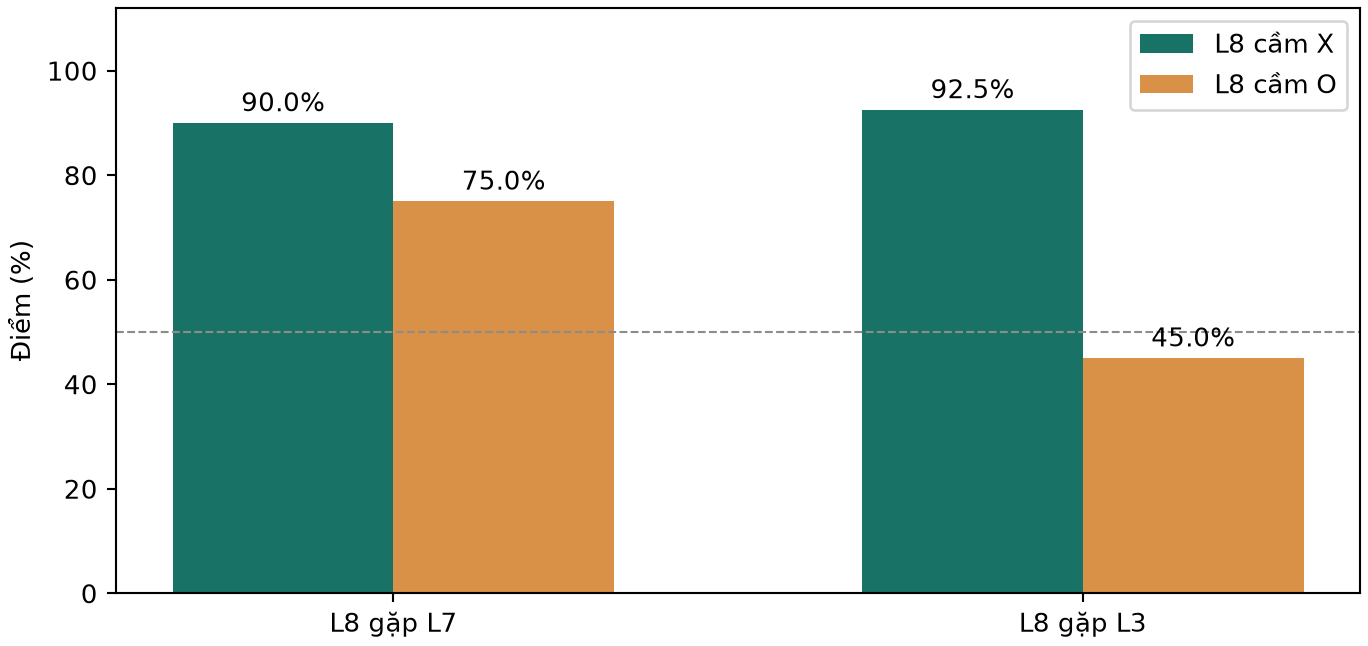
\includegraphics[width=.84\textwidth]{ban-mo-rong/hinh/mau.png}
\caption{Điểm theo màu của L8 trong hai lượt đấu. Mỗi cột tính hòa nửa điểm.}
\end{figure}

Trong 20 ván L7--L8, X thắng 11 ván, O thắng 8 và hòa 1. X hơn O 15 điểm phần trăm về tỷ lệ thắng thuần. Bootstrap theo 10 khai cuộc cho khoảng tham khảo từ $-20$ đến $+50$ điểm phần trăm. Khoảng đi qua 0, nên mẫu hiện tại chưa xác định được dấu của hiệu ứng đi trước một cách ổn định. Chênh lệch theo màu của L8 trước L3 lớn hơn trong phép thử đó. Kết quả có thể phụ thuộc đối thủ, tập khai cuộc và lối chơi; E3 tự đấu từng cấp vẫn là một khảo sát riêng.

Quy tắc phát lại chỉ kiểm chứng tình huống có bằng chứng bằng bitboard: thắng ngay, bỏ lỡ thắng ngay, bỏ chặn duy nhất, chặn bắt buộc và tạo hai ô thắng khi đối thủ không có nước thắng tức thì. Các tình huống không thể cứu ngay ở nước kế tiếp được xếp riêng thay vì quy thành lỗi của nước vừa đánh. Ván 13 của lượt L7--L8 minh họa trường hợp L7 đi B5 khi cần chặn G4. Phụ lục ván đấu ghi mã ván, thế cờ, các lựa chọn và trình tự nước để kiểm tra lại.

Hai lượt đối đầu khác nhau rõ về mức độ đảo kết quả khi đổi màu. Trước L7,
L8 thắng cả hai ván trên sáu khai cuộc, thắng một và hòa một trên một khai cuộc,
và chia thắng--thua trên ba khai cuộc. Trước L3, L8 thắng cả hai ván trên năm
khai cuộc, thắng--hòa trên năm khai cuộc và chia thắng--thua trên mười khai cuộc.
Không có khai cuộc nào trong hai lượt mà L8 thua cả hai màu. So sánh theo cặp
làm rõ rằng điểm cao khi cầm X không tự chuyển thành lợi thế tương tự khi cầm O.

\begin{table}[H]
\centering\small
\begin{tabular}{@{}lrrrrr@{}}
\toprule
Đối thủ của L8 & Khai cuộc & X thắng & O thắng & Hòa & Chênh X--O \\
\midrule
L7 & 10 & 11 & 8 & 1 & 15,0 đpt \\
L3 & 20 & 27 & 8 & 5 & 47,5 đpt \\
\bottomrule
\end{tabular}
\caption{Tỷ lệ đi trước đo từ kết quả tuyệt đối của X và O, gộp tác tử trong từng đối sánh. Chênh lệch là tỷ lệ thắng thuần, không tính hòa nửa điểm.}
\label{tab:mau-gop}
\end{table}
Ở cặp L8--L3, khoảng bootstrap mô tả của chênh lệch X--O là 20,0 đến 72,5
điểm phần trăm. Kết quả này hỗ trợ lợi thế màu trên mẫu đang xét, nhưng không
thay thế E3 vì hai tác tử có kiến trúc khác nhau và cùng dùng một corpus khai cuộc.

\paragraph{Ván 13: L7 bỏ nước chặn duy nhất trước L8.}
Khai cuộc 48, L7 cầm X. Trước nước 35, O có quân ở G3, G5, G6 và G7;
G4 là ô thắng ngay duy nhất của O. X chọn B5. O đặt G4 ở nước 36 để nối
G3--G7. Kiểm tra luật xác nhận G4 chặn được đe dọa trực tiếp; từ đó chưa
suy ra rằng X sẽ thắng hoặc hòa nếu chặn đúng.

\paragraph{Ván 26: L8 cũng có sai sót chiến thuật trước AlphaBeta.}
Khai cuộc 6, AlphaBeta cầm X và L8 cầm O. Ở nước 20, O đi C8 khi E7 là ô
chặn duy nhất. X đi E7 ở nước 21, hoàn thành dãy D7--H7. Hai ví dụ dùng cùng
quy tắc kiểm chứng, nên lỗi được mô tả theo thế cờ thay vì theo tác tử yêu thích.
Để biết lỗi hiếm hay thường gặp, Bảng~\ref{tab:co-hoi-chien-thuat} đếm cả cơ hội thực hiện
nước đúng. Một cơ hội chặn chỉ được tính khi đối thủ có đúng một ô thắng và
bên đang đi không có ô thắng ngay. L8 chặn đúng toàn bộ 46 lần trước L7, nhưng
bỏ chặn 3/137 lần trước L3. L3 chặn đúng cả 84 cơ hội trong cùng đối sánh.
Các tỷ lệ mô tả những thế thực sự xuất hiện; hai tác tử chưa được đặt vào
cùng tập thế phòng thủ, nên không xếp hạng chúng chỉ dựa trên các tỷ lệ này.

\begin{table}[H]
\centering\small
\begin{tabular}{@{}llrrr@{}}
\toprule
Đối sánh & Tác tử & Phải chặn & Bỏ chặn & Thắng ngay thành công \\
\midrule
L7--L8 & L7 & 47 & 4 & 3/3 \\
L7--L8 & L8 & 46 & 0 & 16/16 \\
L3--L8 & L3 & 84 & 0 & 10/10 \\
L3--L8 & L8 & 137 & 3 & 25/25 \\
\bottomrule
\end{tabular}
\caption{Kiểm tra cơ hội chiến thuật bằng cách phát lại các nước sau chuỗi khai cuộc. Cột cuối ghi số nước thắng ngay đã chọn trên tổng số cơ hội thắng ngay.}
\label{tab:co-hoi-chien-thuat}
\end{table}

\section{Phân tích lỗi}
\paragraph{Phương pháp.}
Với mọi ván MCTS thua trong A3 và A4 (tổng 2\,381 ván), script \texttt{report/scripts/phan\_tich\_loi\_mcts.py} phân loại lỗi bằng engine (\texttt{winning\_squares}), không đoán tay. Tại nước cuối của MCTS, nếu đối thủ có đúng một ô thắng ngay mà MCTS không chặn thì là ``bỏ sót chặn năm''. Nếu đối thủ đã có từ hai ô thắng (tứ hở, đòn kép) thì ván đã thua, và script xét nước kế cuối: đối thủ có nước tạo từ hai ô thắng mà MCTS không ngăn là ``bỏ sót chặn ba hở / đòn kép''.

\begin{table}[H]
  \centering
  \footnotesize
  \begin{tabular}{lrrr}
    \toprule
    \textbf{Cấu hình} & \textbf{Ván thua} & \textbf{Bỏ sót chặn ba hở / đòn kép} & \textbf{Bỏ sót chặn năm} \\
    \midrule
    A3, 100 mô phỏng   & 400 & 92{,}5\% & 7{,}5\% \\
    A3, 400 mô phỏng   & 400 & 91{,}2\% & 8{,}8\% \\
    A3, 1600 mô phỏng  & 400 & 88{,}5\% & 11{,}5\% \\
    A3, 6400 mô phỏng  & 381 & 92{,}9\% & 7{,}1\% \\
    A4, \texttt{random} (800) & 400 & 89{,}8\% & 10{,}2\% \\
    A4, \texttt{light} (800)  & 400 & 65{,}2\% & 34{,}8\% \\
    \bottomrule
  \end{tabular}
  \caption{Phân loại lỗi trong các ván MCTS thua. Một vài ván (dưới 2\%) thuộc lớp ``bỏ sót chặn năm ở nước kế cuối'' và được tính vào cột cuối.}
  \label{tab:loi-mcts}
\end{table}

Hai nhận xét rút ra từ Bảng~\ref{tab:loi-mcts}. Thứ nhất, lỗi chủ đạo ở mọi mức mô phỏng là không ngăn đe doạ kép sớm (khoảng 90\%); tăng mô phỏng từ 100 lên 6400 không đổi tỷ lệ này, khớp với thảo luận ở A3/A4 rằng cây quá nông cho cấu trúc 4 ply. Thứ hai, với rollout \texttt{light} tỷ lệ bỏ sót chặn năm \emph{tăng} lên 34{,}8\%, dù rollout đã biết chặn. Nguyên nhân là rollout chỉ chặn bên trong mô phỏng, còn ở gốc cây thì thống kê thăm quá thưa nên nước chặn bắt buộc có thể không được chọn.

\subsection{Kiểm chứng A8: chiến thuật tại gốc trên tập giữ riêng}

\section{Thảo luận}
Các biến thể tìm kiếm cần được so sánh đồng thời về điểm và chi phí. Kết quả 82,5\%
của L8 trước L7 là bằng chứng về cặp checkpoint đã đo. Cỡ mẫu 20 ván và sự trùng khai cuộc
với giai đoạn gating giới hạn khả năng ngoại suy. L8 ghi 68,75\% trước AlphaBeta sau khi đổi màu. Để đo phần cải thiện
trước AlphaBeta một cách ghép cặp, cần cho L7 và L8 gặp cùng phiên bản L3, dùng cùng
khai cuộc, đổi màu, rồi bootstrap chênh lệch điểm trên từng khai cuộc.
So sánh thời gian mỗi nước cũng cần giữ nguyên loại máy, backend và cách khởi tạo.
Kết quả xác định sức chơi trên các đối sánh đã chạy, chưa xác định sức chơi tối ưu. Nên tái kiểm định trên bộ khai cuộc giữ riêng trước khi dùng các mức điểm này
để xếp hạng chung.

\subsection{Giải trên khai cuộc giữ riêng}
\subsection{So sánh PUCT Python, Cython và gom suy luận trên GPU}
